\documentclass[preview]{standalone}
\usepackage{caption}
\usepackage{tikz}
\usetikzlibrary{fit, arrows}
\captionsetup[figure]{labelformat=empty}

\begin{document}
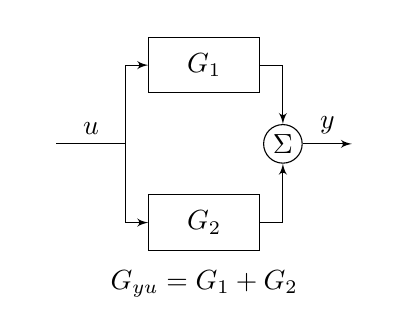
\begin{tikzpicture}[auto, node distance=1cm,>=latex']
  \tikzstyle{block} = [draw, rectangle, minimum height=2em, minimum width=4em]
  \tikzstyle{sum} = [draw, fill=white, circle, inner sep=0.5mm]
  \tikzstyle{tmp} = [coordinate]
  \node (input) {};
  \node [tmp, right of=input] (split) {};
  \node [tmp, right of=split] (mid) {};
  \node [block, above of=mid] (G1) {$G_1$};
  \node [block, below of=mid] (G2) {$G_2$};
  \node [sum, right of=mid] (sum) {$\Sigma$};
  \node [right of=sum] (output) {};
  \node [fit=(input) (mid) (sum) (G1) (G2) (output), label=below:{$G_{yu}=G_1+G_2$}] {};

  \draw (input) -- node {$u$} (split);
  \draw [->] (split) |- node {} (G1);
  \draw [->] (split) |- node {} (G2);
  \draw [->] (G2) -| node {} (sum);
  \draw [->] (G1) -| node {} (sum);
  \draw [->] (sum) -- node {$y$} (output);
\end{tikzpicture}
\end{document}
